\section{Von Neumannovy principy, blokové schéma Von Neumannova počítače. Rozdíl mezi Von Neumannovou, harvardskou a modifikovanou harvardskou architekturou. Procesory CISC a RISC. Rozdíl mezi obvodovým a mikroprogramovým řadičem. Řetězové zpracování instrukcí (pipelining), skokový a datový konflikt. Jak se liší a pro jaké typy úloh je určen mikroprocesor pro všeobecné použití, mikrokontrolér, signálový procesor a signálový kontrolér (DSC), SoC (System on a Chip), ASIC.}
\subsection{Von Neumnnova architektura}
\subsubsection*{Hlavní myšlenka}
Instrukce programu jsou reprezentovány binárními signály a jsou uloženy v paměti počítače spolu s daty. \\
\subsubsection*{Principy}
Principy:
\begin{itemize}
    \item Předpis pro řešení úlohy je převeden na posloupnost instrukcí
    \item Intrukce a data se nacházejí ve stejné paměti
    \item Instrukce ani data nejsou explicitně označeny
    \item Paměť je rozdělena na stejně velká paměťová místa nazývaná adresy
    \item V instrukcích není uvedena hodnota operandu, ale jeho adresa
    \item instrukce se provádějí sekvenčně
    \item Toto sekvenční provádění lze narušit instrukcemi typu skok
\end{itemize}

\begin{figure}[h!]
    \centering
    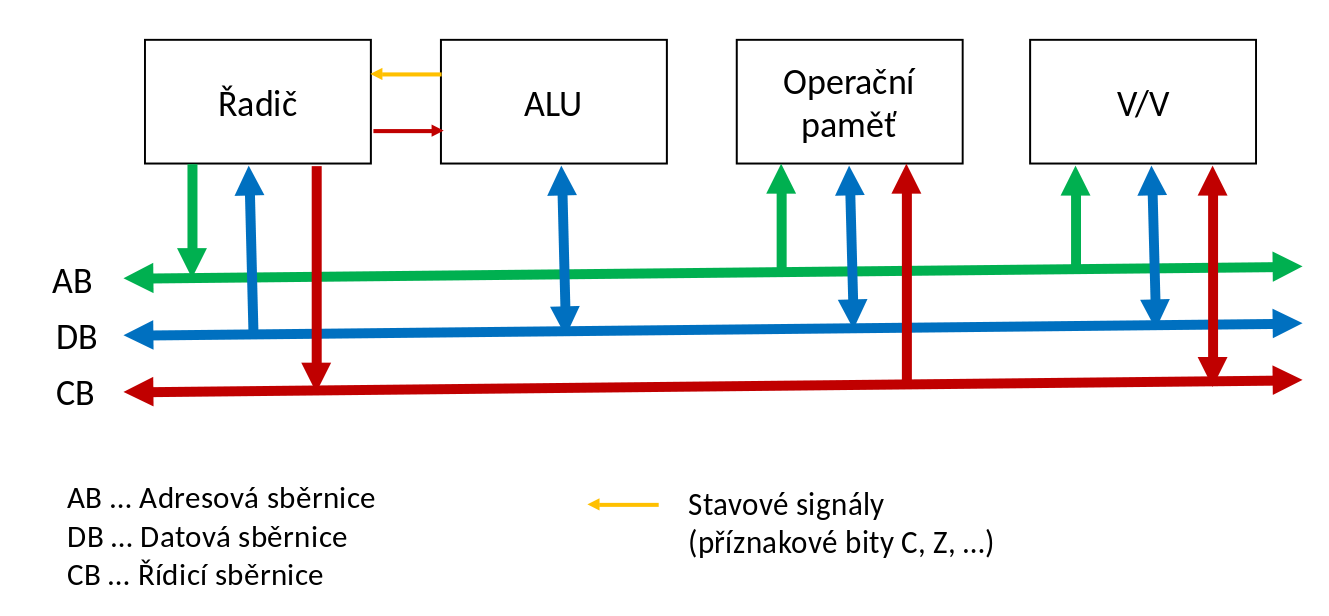
\includegraphics[width = \textwidth]{img/VonNeumann.png}
\end{figure}

\subsubsection*{Řadič}
Řídí činnost ostatních částí počítače. \\
Implementuje instrukční sadu. \\
Vstupy:\\
\begin{itemize}
    \item Signály z dekodéru instrukcí - dekóduje se část instrukce označována jako operační znak
    \item Signály generované ALU - Příznaky, přetečení, nulový výsledek, záporný výsledek
    \item Signál žádosti o obsluhu přerušení
\end{itemize}
Výstupy:\\
\begin{itemize}
    \item Čtení nebo zápis do paměti
    \item Čtení nebo zápis do periferie
    \item Signály ALU, určující kterou operaci má provést
\end{itemize}

\subsubsection*{ALU}
Aritmeticko-logická jednotka.\\
Provádí aritmetické operace(+,-,/,*), logické operace(AND,OR,NOT) a operace porovnání(>,<,=)\\
Řadič a ALU tvoří CPU. Integrací řadiče, ALU a registrů na jeden čip vzniká mikroprocesor.

\subsubsection*{Operační paměť}
Místo uložení dat a instrukcí.\\
Společná paměť pro instrukce a data. Jsou uloženy v jednom paměťovém prostoru.\\
U mikrokontrolerů jsou v instrukce v paměti FLASH a proměnné v paměti RAM, ale obě jsou připojeny ke stejným sběrnicím(AB,CB,DB)

\subsubsection*{V/V}
Slouží pro komunikaci s okolím.\\
Člověkem - klávesnice, myš, obrazovka. \\
Strojem, přístrojem či technologickým procesem - I/O, A/D, D/A převodníky a k nim akční členy - snímače. \\
S ostatními počítači a zařízeními pomocí sítě - Ethernet, WiFi moduly. \\
Umožňují ukládání dat na disky(SSD, HDD). \\

\subsubsection*{Registry}
Typy registrů:
\begin{itemize}
    \item Pracovní registr
          \begin{itemize}
              \item Ukládají operandy z ALU a výsledky z ALU
              \item Rychlejší než operační paměť
              \item Původně jeden registr nazývaný akumulátor
          \end{itemize}
    \item Stavový registr
          \begin{itemize}
              \item Skupina klopných obvodů ovládaných ALU
              \item Uchovávají stav ALU mezi instrukcemi
              \item Příznaky přetečení/výpůjčky, nulového či záporného výsledku
              \item Předcházející instrukce příznaky nastaví, následující využije
          \end{itemize}
    \item Programový čítač
          \begin{itemize}
              \item Zajišťuje sekvenční provádění instrukcí a provádění skoků
              \item V průběhu zpracování instrukce se nastaví tak aby obsahoval adresu následující instrukce
          \end{itemize}
\end{itemize}
Řídící a stavový registr bývají spojeny do jednoho řídícího stavového registru.\\

\subsubsection{Cyklus počítače}
Celý cyklus práce počítače se dělí na tyto opakující se části.
\begin{enumerate}
    \item Intruction fetch - načtení instrukce z paměti
    \item Intruction decode - dekódování instrukce
    \item Operand fetch - načtení operandu z registrů
    \item Intruction expectation
    \item Write-back (Result store) - uložení výsledku
    \item Test, není-li požadavek na přerušení
\end{enumerate}
Nemusí se nutně vykonávat všechny tyto fáze.\\
Povinné fáze jsou pouze 1,2,4.

\subsection{Rozdíly mezi VonNeumannovou, harvardskou a modifikovanou harvardskou architekturou}
\subsubsection*{Von Neumannova architektura}
Společná paměť pro instrukce a data. \\
Existuje jedna datová a jedna adresová sběrnice. \\
Pomalejší oproti HA a MHA kvůli nutnosti číst instrukce nebo operand. \\
Výhoda spouštění programů z disků, jednoduchá změna počítače. \\
Dobře využitelná paměť. \\
Poloviční počet sběrnic oproti HA. Jednodušší konstrukce. \\
\begin{figure}[h!]
    \centering
    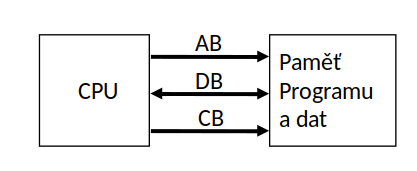
\includegraphics[]{img/VNporovnani.png}
\end{figure}

\subsubsection{Harvardská architektura}
Oddělena paměť dat a programu. To umožňuje číst obě zaráz a urychluje práci.\\
Může být různě adresována datová paměť a programová paměť.\\
Bezpečnější, nelze si poškodit program přepsáním jeho paměti.\\
Dvojnásobek sběrnic oproti VN, technilogicky velký problém. \\
Nevyužitou část paměti nejde použít pro program a naopak. Z toho plyne, že je nižší efektivita využití paměti. \\
Využívá se u signálových procesorů, jinak moc ne.\\
\begin{figure}[h!]
    \centering
    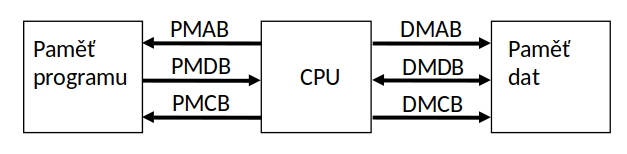
\includegraphics[width = \textwidth]{img/HAporovnani.png}
\end{figure}

\subsubsection*{Modifikovaná harvardská architektura}
Stejně jako HA 2 paměti. S rozdílem toho, že jedna je čistě pro data a druhá pro data a program.\\
Umožňuje číst 2 operandy zároveň díky rozmístění paměti. Toto umožňuje operaci Multiply and accumulate. \\
Využívá se u signálových procesorů a kontrolerů. \\

\begin{figure}[h!]
    \centering
    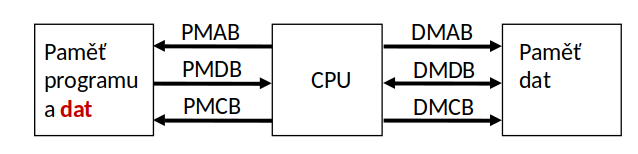
\includegraphics[width = \textwidth]{img/MHAporovnani.png}
\end{figure}

\subsection{Obvodový a mikroprogramový řadič}
\subsubsection*{Obvodový řadič}
Synchronní konečný stavový automat.\\
Logické členy a klopné obvody. \\
Umožňuje malou sadu jednoduchých instrukcí. \\
Výhodou je jednoduchost a malý počet součástek. \\
Nevýhodou je nutnost složité operace rozdělovat na více instrukcí. \\

\subsubsection*{Mikroprogramový řadič}
KSA, jehož paměť je tvořena pamětí mikroprogramu. \\
Implementuje složité instrukce za cenu složitosti řadiče. \\
Složité instrukce není možné přímo provést, proto jsou rozděleny na mikroinstrukce. \\
Posloupnost mikroinstrukcí, jimiž se vykoná instrukce se nazývá mikroprogram. \\
Mikroprogramy pro jednotlivé instrukce jsou uloženy v paměti mikroprogramu. \\
Toto zvyšuje složitost řadiče a počet cyklů potřebných na provedení instrukce. \\
Nutno operovat v nižších frekvencích kvůli problému s odvodem tepla. \\

\subsection{Procesory CISC a RISC}
\subsubsection*{CISC}
Complex instruction set computer. \\
Složité instrukční sady, přizůsobené tak aby realizovaly příkazy programovacího jazyka. \\
Používá mikroprogramový řadič. \\
Stovky instrukcí. \\
Přesun složitosti z SW do HW. \\

\subsubsection*{RISC}
Reduced instruction set computer. \\
Malý počet jednoduchých instrukcí. \\
Vyšší nároky na překladače z programovacích jazyků. \\
Instrukce mají konstatní délku a jednotný formát, který vymezuje počet bitů v instrukci. \\
Obvodový řadič. \\
Velký počet registrů(16+), to snižuje nutnost častého přístupu do operační paměti. \\
Jediné instrukce, které mají povoleno interagovat s pamětí jsou \texttt{load} a \texttt{store}, load z paměti do registru, store naopak. Ostatní instrukce pracují pouze s registry.\\
V každém hodinovém taktu dokončena jedna instrukce. \\
Používá pipelining. \\

\subsubsection*{Post-RISC}
Kombinace CISC a RISC. \\
Rozšiřuje RISC o instrukce, které lze provádět rychle. \\
Hluboká pipeline až 10 kroků. \\
Více ALU pracujících paralelně. \\

\subsection{Řetězové zpracování instrukcí - pipelining}
Efektivnější využití času. \\
Každá fáze využívá jinou část CPU -> návrh procesoru pro paralelní práci na jeho částech. \\

\begin{figure}[h!]
    \centering
    \begin{minipage}[b]{0.4\textwidth}
        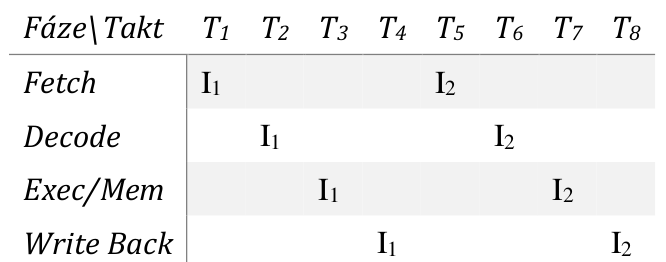
\includegraphics[width=\textwidth]{img/sekv.png}
    \end{minipage}
    \hfill
    \begin{minipage}[b]{0.4\textwidth}
        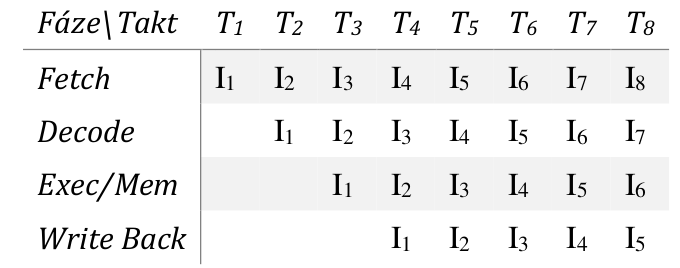
\includegraphics[width=\textwidth]{img/pipeline.png}
    \end{minipage}
\end{figure}

Doba exekuce instrukcí, kde k je počet fází:
\begin{center}
    Pipelining: $N = k + (n-1)$\\
    Sekvenční: $M = n \cdot k$ \\
    Koeficient zrychlení: $S_k = \frac{M}{N} = \frac{n \cdot k}{n + n-1}$
\end{center}

\subsection{Skokový konflikt}
Při instrukci větvení nebo přerušení. Ve chvíli kdy se začne provádět skok jsou v řetězci rozpracované instrukce. Řetězec tudíž musí být vyprázdněn a znovu naplněn, což vede ke snížení efektivity.\\
Řešení:
\begin{itemize}
    \item Predikce skoků
          \begin{itemize}
              \item Statická - nebere v úvahu historii provádění příslušné operace skoku. Například při provádění cyklu se skok provede vždy, instrukce obsahuje bit, který nastaví překladač (překladač odhaduje pravděpodobnost skoku)
              \item Dynamická - snaží se předpovědět skoky na základě chování programu v minulosti. Například provedl-li se skok při minulé exekuci dané instrukce počítá se, že se provede znovu. Procesor musí být vybaven spekulativní jednotkou
          \end{itemize}
    \item Použití dvou řetězců - 2 řetězce, jeden pro sekvenční provádění a druhý pro skoky.
\end{itemize}

\subsection{Datový konflikt}
Pokud instrukce pracuje s operandem z předchozí instrukce, která se však ještě nedokončila. \\

\begin{figure}[h!]
    \centering
    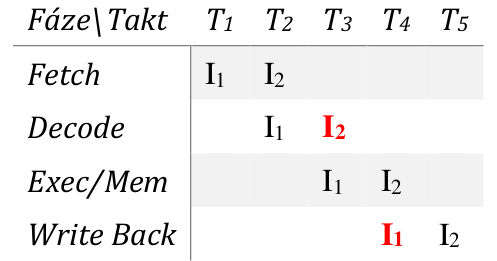
\includegraphics[scale = 0.4]{img/datKonf.png}
\end{figure}

Řešení:
\begin{itemize}
    \item Překladač řadí instrukce tak aby ke konfliktu nedošlo.
    \item Procesor detekuje konflikt a pozastaví konání $I_2$. Snižuje účinost řetězení.
    \item Procesor detekuje konflikt a změní pořadí instrukcí. Náročné na konstrukci procesoru.
\end{itemize}

\subsection{Superpipelined procesor}
Procesor rozdělený na subprocesory, které zpracovávají instrukce jako řetězec. \\
Subprocesory je možné dělit na subbloky, které tvoří řetězce subprocesorů. \\

\subsection{Mikroprocesor, mikrokontrolér, signálový procesor, signálový kontroler,SOC, ASIC}
\subsubsection{Mikroprocesor pro všeobecné využití}
Na jednom čipu ALU, řadič, registry, případně cache a MMU.\\
Velký výpočetní výkon a paměťový prostor.\\
Stolní PC, notebooky, servery.\\
Modifikace pro telefony a tablety, optimalizovány na nízkou spotřebu, nižší výkon a paměť. \\

\subsubsection*{Mikrokontrolér}
Základní stavební kámen vesvných zařízeních. \\
Na jednom čipu procesor (řadič, ALU, registry, případně cache a MMU), paměti RAM a FLASH, řadič přerušení a periferie.\\
Menší výkon a paměť.\\
Určen pro embedded aplikace, spotřební elektronika, průmysl, automobily, řídící aplikace. \\

\subsubsection*{Signálový procesor - DSP}
Vznikly pro číslicové zpracování signálů v reálném čase a spektrální analýzu. \\
Vyžadují rychlé provádění specifických výpočetních operací, ale nepotřebují moc paměti. Například multiply and accumulate, v podstatě konvoluce, součin dvou parametrů a přičtení k proměnné.\\
Méně periferií než mikrokontroléry. \\
Dělí se na 2 typy:
\begin{itemize}
    \item S pevnou řádovou čárkou - jednodušší, levnější, algoritmy se hůře implementují
    \item S plovoucí řádovou čárkou, dražší, ale jednodušší implementace
\end{itemize}

\subsubsection*{Signálový kontroler - DSC}
Kombinace DSP a mikrokontroleru.\\
Má více periferií oproti DSP. \\
Využití pro výkonovou elektroniku. Měniče, vektorové řízení motorů.\\

\subsubsection*{System on a chip - SoC}
Integrovaný obvod, který zahrnuje všechny části počítače na jeden čip. \\
Digitální, analogové, rádiové, smíšené obvody na jednom čipu. \\

\subsubsection*{ASIC}
Integrovaný obvod navržený pro jednu aplikaci.\\
Většinou digitální, hromadná výroba.\\


\section{Rozdíl mezi izolovanými a paměťově mapovanými periferiemi. Způsoby obsluhy V/V: aktivní čekání, přerušení, DMA.
  Přerušení: řadič přerušení, činnost procesoru při zahájení obsluhy přerušení a návratu z přerušení, tabulka vektorů přerušení. Asynchronní a synchronní přerušení. Maskovatelné, nemaskovatelné a pseudomaskovatelné přerušení. Vnořené přerušení. RESET, činnost procesoru po RESETu.}
\subsection{Izolované a paměťově mapované periferie}
\subsubsection{Izolované}
Periferie využívají samostatný adresový prostor oddělený od adresového prostoru operační paměti.\\
Pro přístup k izolovaným periferiím se používají speciální instrukce.\\
Intel procesory mají společnou AB a DB pro periferie i operační paměť. Intrukce IN a OUT.

\subsubsection*{Paměťově mapované}
Periferie se nacházejí ve stejném paměťovém prostoru jako operační paměť. \\
Pro přístup k periferiím se používají stejné instrukce jako pro přístup k operandům v operační paměti.\\
\subsection{Způsob obsluhy V/V}
\subsubsection*{Řídící registry periferií}
Různé periferie se značně liší, ale práce s nimi je do jisté míry podobná.\\
Z hlediska programátora jsou důležité registry periferií, které se podle funkce dají rozdělit:
\begin{itemize}
    \item Konfigurační (řídící) registry - slouží pro nastavení režimu fungování periferie.
    \item Stavové (příznakové) registry - obsahují příznakové bity (flagy), které signalizují stav periferie (např. stavový registr A/D převodníku obsahuje bit signalizující dokončení převodu)
    \item Datové registry - slouží pro vyčítání nebo ukládání dat, které periferie zpracovává
\end{itemize}

\subsubsection*{Obsluha pomocí aktivního čekání - busy waiting, pooling}
Procesor odstartuje V/V operaci zápisem do řídícího nebo datového registru a pak ve smyčce testuje, zda-li byla operace dokončena nebo došlo k chybě - to značí příslušný bit (flag).\\
Velká nevýhoda je, že během čekání ve smyčce procesor nemůže provádět jinou užitečnou činnost => plýtvání času.\\
V embedded systémech hrozí, že dojde k promeškání důležité události (např. nárust tlaku v nádobě => havárie).\\
Jediná výhoda je jednoduchá implementace, využívá se při testování u vývoje periferií.\\

\subsubsection*{Obsluha pomocí přerušení}
Procesor odstartuje V/V operaci zápisem do řídícího nebo datového registru. \\
Nečeká na dokončení operace, ale provádí jinou užitečnou činnost.\\
Po dokončení operace nebo při chybě periferie generuje požadavek na přerušení.\\
Procesor rozpozná požadavek na přerušení a dočasně přeruší provádění aktuálního kódu a vykoná kód obslužné rutiny přerušení pro danou periferii. \\
Po vykonání obslužné rutiny se procesor opět vrátí k vykonávání kódu, který prováděl před přechodem do přerušovací rutiny.\\

\subsubsection*{Obsluha pomocí DMA}
Některé periferie (např. řadiče disků) obsahují vyrovnávací paměti.\\
Při provádění V/V operací je třeba přenášet větší množství bytů mezi operační pamětí a vyrovnávací pamětí periferie. \\
Je výhodné, aby přenos dat probíhal bez účasti procesoru a procesor mohl provádět jinou užitečnou činnost. Aby toto bylo možné musí v počítači být řadič sběrnic - DMA. Během přenosu dat CPU uvolní sběrnice a ty převezme řadič DMA. DMA generuje adresy a řídící signály jako MEMR a MEMW.
Před zahájením DMA přenosu musí procesor na DMA nakonfigurovat:
\begin{itemize}
    \item Počáteční adresu v operační paměti.
    \item Počáteční adresu v paměti periferie.
    \item Směr přenosu.
    \item Počet přenášených bytů.
\end{itemize}

\subsection{Přerušení}
\subsubsection*{Použití přerušení}
Používá se pro obsluhu neodkladných událostí. \\
Při požadavku na přerušení procesor přeruší aktuálně prováděný kód a provede kód obsluhující událost a vrátí se zpět.\\
Kód obsluhy se nazývá obslužná rutina přerušení.\\
Používá se pro obsluhu periferií, nebo k ošetření výjimečných situací jako chyby a havarijní stavy (např. dělení nulou, chyba ochrany paměti, pokles napájecího napětí atd.).\\
Přerušení lze také vyvolat softwarově pomocí příslušné instrukce. Používá se pro přístup ke službám jádra operačního systému. Na některých procesorech je to jediný způsob, jak lze přejít z uživatelského módu na mód supervisor (v němž běží jádro operačního systému)

\subsubsection*{Řadič přerušení}
Počítač obvykle používá více V/V periferií, které mohou generovat požadavky na přerušení.\\
Jednotlivé zdroje přerušení jsou připojeny na vstupy bloku počítače nazývaného řadič přerušení.\\
Aby procesor mohl určit zdroj přerušení, je ke každému zdroji přiřazeno celé kladné číslo. Periferie nastaví aktivní úroveň signálu na vstup řadiče a ten zašle číslo přerušení. Periferie mají z hlediska obsluhy různou prioritu, podle toho se řadič rozhoduje, co oznámí procesoru jako první, když je současně generováno víc požadavků.\\
Priorita buď softwarově nebo hardwarově, softwarovou můžeme měnit zápisem do řadiče.\\
Dnešní počítače vybavené sběrnicí PCI Express nepoužívají dedikované vodiče pro komunikaci mezi řadičem a procesorem, periferie posílají požadavek na obsluhu jako zprávu po sběrnici PCIe. Zpráva je posílána na speciální adresu v paměťovém prostoru. Tento způsob přerušení se nazývá MSI ( Message Signaled Interrupts).

\subsubsection*{Činnost procesoru při obsluze přerušení}
Při příchodu požadavku na asynchronní nebo softwarové přerušení procesor dokončí prováděnou instrukci. \\
Na konci instrukčního cyklu procesor testuje, jestli není požadavek na obsluhu přerušení, pokud je, tak procesor zahájí obsluhu:
\begin{enumerate}
    \item Uloží do zásobníku návratovou adresu
    \item Uloží do zásobníku obsah stavového registru
    \item Některé procesory ukládají do zásobníku obsah pracovních registrů
    \item V příznakovém registru nastaví bit I, čímž zakáže přerušení. Během provádění obslužné rutiny jsou maskovatelná přerušení zakázána, pokud je programátor v přerušovací rutině explicitně nepovolí
    \item Procesor na základě čísla přerušení stanoví adresu vektoru přerušení. Na adrese vektoru přerušení se musí nacházet adresa první instrukce obslužné rutiny
    \item Procesor vyzvedne adresu první instrukce z vektoru přerušení a vloží ji do programového čítače - tím se začne provádět obslužná rutina
\end{enumerate}
Poslední instrukce obslužné rutiny přerušení musí být instrukce návratu z přerušení (RTI), která zajistí, že procesor:
\begin{itemize}
    \item Pokud procesor uložil obsah pracovních registrů, obnoví jejich obsah
    \item Obnoví ze zásobníku obsah stavového registru - tím se povolí maskovatelná přerušení (nastavení bitu I)
    \item Vyzvedne ze zásobníku návratovou adresu a vloží ji do programového čítače, v případě asynchronního přerušení procesor pokračuje následující instrukcí, u výjimek (např. dělení nulou) se restartuje instrukce, která výjimku způsobila
\end{itemize}
Pokud má procesor větší množství pracovních registrů, ukládání pracovních by trvalo nepřijatelně dlouho, přitom by programátor nebo překladač obsah některých registrů v přerušovací rutině nemodifikoval. Proto procesory s větším množství registrů tyto registry automaticky neukládají a je odpovědnost programátora nebo překladače uložit ty registry, které se budou modifikovat.\\
Existují procesory, které mají pracovní registry zdvojené a jen se přepíná mezi hlavními a stínovými(pro rutinu) registry. Přepínání je rychlé, ale velmi náročné na konstrukci. Toto řešení je dnes spíše výjimkou. \\

\subsubsection*{Vektor přerušení}
Adresa kde se nachází první instrukce obslužné rutiny.\\
Každý zdroj přerušení má svůj vektor přerušení.\\

\subsubsection*{Tabulka vektorů přerušení}
Oblast paměti kde jsou za sebou umístěny vektory přerušení.\\
Číslo vektoru je indexem tabulky vektorů.\\
Řadič předá procesoru číslo vektoru přerušení, procesor vynásobí číslo vektoru přerušení velikostí vektoru přerušení a výsledek přičte k adrese začátku tabulky vektorů přerušení.\\
Počáteční adresa tabulky bývá u jednoduchých procesorů daná výrobcem napevno, složitější na to mají speciální registr, kde se napíše námi zvolená adresa.

\subsubsection*{Asynchronní a synchronní přerušení}
\begin{itemize}
    \item Asynchronní
          \begin{itemize}
              \item nejsou synchronizovány s prováděním instrukcí v CPU
              \item jsou vyvolány asynchronními událostmi
              \item typické zdroje jsou V/V periferie - dokončení AD převodu, doběhnutí časovače, příjem ethernet rámce, zmáčknutí klávesy, detekce poklesu napětí
          \end{itemize}
    \item Synchronní
          \begin{itemize}
              \item Generována v důsledku provádění určitých instrukcí v přesně definované fázi zpracování dané instrukce.
              \item Přerušní generují instrukce softwarového přerušení a výjimky
              \item Výjimky jsou generovány kontrolními obvody počítače, když dojde k chybě v provádění instrukce. Typické výjimky jsou dělení nulou, pokus o exekuci neznámé či ilegální instrukce, noprávněný pokud o přístup k paměti
          \end{itemize}
\end{itemize}

\subsubsection*{Maskovatelná přerušení}
Přerušení lze povolit nebo zakázat obvykle nastavením (vynulováním) bitu I v příznakovém registru.\\
Např. Program provádí úsek kódu kde pracuje s proměnnými, které používá přerušovací rutina, před začátkem práce s těmito proměnnýma zakáže přerušení a provede manipulaci a pak opět povolí přerušení.\\

\subsubsection*{Nemaskovatelná přerušení}
Kritické události jako porušení paměti nebo výpadek napájení je však třeba obsloužit vždy. \\
Tyto přerušení musí být povolena vždy a nesmí být možnost je zakázat.\\
Například porušení paměti či výpadek napájení. \\

\subsubsection*{Pseudomaskovatelná přerušení}
U nemaskovatelných vznikal problém při zahájení činnosti procesoru po RESETu. Obsluha přerušení vyžaduje minimálně nastavení ukazatele zásobníku na adresu začátku zásobníku  v paměti RAM. Vyvolání přerušení v okamžiku, kdy není nastaven ukazatel může způsobit zhroucení celého systému. Proto je potřeba po dobu základní inicializace zabránit obsluze jakýchkoliv přerušení, tedy i nemaskovatelných. \\
Toto přerušení je po resetu zakázáno, ale po inicializaci systému se přerušení povolí a do dalšího resetu jej nejde zakázat a chová se jako nemaskovatelné. \\

\subsubsection*{Vnořená přerušení}
Může nastat situace, kdy procesor provádí obslužnou rutinu přerušení a během ní dojde požadavek na další přerušení. \\
Pokud mají stejnou prioritu, tak se první provede jedna a pak až druhá obsluha.\\
V praxi to tak ale většinou není, většinou jedno přerušení má větší prioritu. Takže uprostřed prvního přerušení se provede druhé přerušení (vnořené) a po vykonání se vrátí k prvnímu a to se dokončí.\\
\subsection{RESET a činnost procesoru po RESETu}
RESET procesoru způsobí nastavení procesoru do definovaného výchozího stavu.\\
Z hlediska uživatele to znamená, že se vynulují pracovní registry a řídící registry se nastaví na výrobcem definované hodnoty.\\
Po uvolnění signálu RESET procesor vyzvedne z definované adresy reset vektor adresu první instrukce a vloží ji do programového čítače.\\
Adresa reset vektoru je definována výrobcem a musí být v pevné paměti.\\
Stejně tak musí být první instrukce uložena v pevné paměti. Dnes uloženy ve FLASH paměti kde je UEFI, které provádí incializaci V/V periferií a zavedení OS.\\
U jednoduchých kontrolerů bývá reset poslední vektor v tabulce přerušení.\\

\section{Princip a vlastnosti pamětí ROM, EEPROM, FLASH. Rozdíl mezi paměťmi NOR FLASH a NAND FLASH. Princip pamětí MRAM a FeRAM.}
\subsection{ROM}
Obsah paměti naprogramován při výrobě a nelze změnit. \\
Pro velké objemy výroby. \\
Buňka tvořena tranzistorem MOSFET zapojeným mezi sloupec a zem. \\
Hradlo tranzistoru je připojeno k řádkovému vodiči. \\
U funkčních trazistorů je mezi hradlem a polovodičem vyleptánan tenká vrstva oxidu křemíku. U nefunkčních je vrstva tlustá. \\
Po vybuzení řádkového vodiče dojde u funkčních tranzitorů k vytvoření indukovaného kanálu a tím ke zkratování sloupce na zem (Úroveň Low - logická 0). U nefunkčních kanál nevznikne, tranzistor je nevodivý a sloupec zůstává na úrovni High - logická 1. \\
Proleptání se dělá pomocí masky, kterou se určí který tranzistor bude 0 a který 1. \\

\subsubsection*{PROM}
Obsah paměti si uživatel jednorázově naprogramuje sám. \\
Pak paměť již nelze měnit. \\

\subsubsection*{Transitor s plovoucím hradlem}
Pokud jsou ve floating gate elektrony tak se zvyšuje potřebný potenciál na aktivaci trazistoru a tudíž se tranzistor neaktivuje a představuje logickou 0. \\
Pokud v ní nejsou elektrony, tranzistor se zaktivuje a tudíž představuje logickou 1. \\
Programování a mazání:
\begin{itemize}
    \item Tunelování elektronů
          \begin{itemize}
              \item Programování: Na source a control gate se přivede zvýšené napětí, na source záporný pól a na CG kladný. Tím jsou elektrony tunelovány skrze tenkou vrstvu izolantu do floating gate a tranzistor je naprogramován na logickou 0
              \item Mazání: Na control gate je přiveden záporný pól a na source kladný, tím se trazistor vybije a změní se na logickou 1.
          \end{itemize}
    \item Lavinová injekce
          \begin{itemize}
              \item Programování: Mezi source a drain se vyvolá velký proud přivedením napětí, elektrony získají velkou energii a mohou opustit kanál. Na control gate se přivede zvýšené napětí, které tahá elektrony z kanálu a ty uvíznou ve floating gate.
              \item Vybíjení: Nelze
          \end{itemize}
\end{itemize}

\begin{figure}[h!]
    \centering
    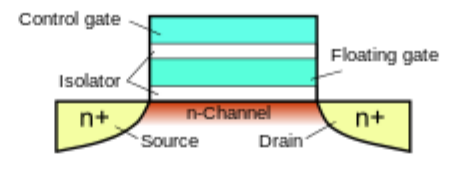
\includegraphics[]{img/FGMOS.png}
\end{figure}
\subsubsection*{EPROM}
Paměťová buňka obsahuje jeden paměťový tranzistor FAMOS (floating Gate Avalanche Injection MOS) - neboli tranzistor s plovoucím hradlem asi. \\
Obsah paměti si uživatel naprogramuje sám, je programovatelná elektricky pomocí zvýšeného napětí. \\
Lze mazat UV zářením. \\
Před programováním musí být paměť vymazána. \\
Počet cyklů programování - mazání je cca desítky. \\

\subsubsection*{EEPROM}
Paměťová buňka složena ze 2 tranzistorů. Paměťový tranzistor splovoucím hradlem. Výběrový tranzistor je MOS, je potřeba abychom mohli měnit obsah každé buňky nezávisle na ostatních. \\
Obsah paměti lze programovat a mazat pomocí elektrických
signálů bez předchozího vymazání. \\
Narozdíl od RAM trvá zápis o několik řádů delší dobu než čtení.     Čtení i zápis v RAM trvá cca nanosekundy, stejně jako čtení paměťového místa EEPROM, zápis ale trvá cca milisekundy. \\
K zápisu i mazání využívá tunelování elektronů. \\
\begin{figure}[h!]
    \centering
    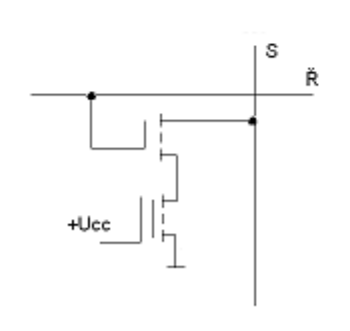
\includegraphics[scale = 0.5]{img/EEPROM.png}
\end{figure}

\subsubsection*{FLASH}
Paměťová buňka tvořena pouze jedním tranzistorem.\\
Speciální druh paměti EEPROM, který umožňuje mazat či zapisovat na více paměťových míst pomocí jedné programovací operace - mazána může být např. celá paměť nebo jen zvolená oblast paměti najednou. \\
Elektricky programovatelná za pomocí lavinové injekce(rychlé), mazání za pomoci tunelování elektronů(pomalé).\\
Mechanismus ochrany proti zápisu - možnost dočasně udělat z paměti read-only. Zápis se pak povolí zapsáním definované sekvence bytů do řídících registrů paměti.\\
Vyšší hustota oproti EEPROM. \\

\subsubsection*{NOR FLASH}
Každý tranzistor je zapojen paralelně ke sloupcovému vodiči. Umožňuje samostatně adresovat každou paměťovou buňku.\\
Programování pomocí lavinové injekce, mazání tunelováním. \\
Rychlé čtení dat s náhodným přístupem. Možnost čtení i zápisu po bytech.\\
Oproti NAND FLASH pomalý zápis a mazání. Pro aplikace kde se data moc nemění.\\
Přímá náhrada ROM, EEPROM, stejné připojení k procesoru.\\
Používá se pro ukládání firmware v embedded systémech a pro ukládání kódu zavaděčů OS(BIOS/UEFI).\\
Každý tranzistor přivedem mezi zem(source) a sloupcový vodič(bit-line).\\
Stačí jeden sepnutý tranzistor aby se bit-line stáhnul do nízké hodnoty. \\

\subsubsection*{NAND FLASH}
Několik paměťových buněk zapojeno do série. Každý paměťový tranzistor nemusí být připojen ke sloupcovému
a zemnímu vodiči -> menší paměťová buňka (hustota informace
až o 45\% vyšší než NOR FLASH).\\
Pro programování i mazání se používá tunelování elektronů.\\
Složitější rozhraní než paměti NOR FLASH. Nelze je přímo připojit ke sběrnicím mikroprocesoru. Čtení s náhodným přístupem je pomalé, proto není možné z paměti přímo provádět kód. \\
Čtení: na všechny tranzistory ve skupině mimo čteného se přivede vyšší než prahové napětí(všechny se sepnou). Na čtený se přivede napěttí vyšší jak práh pro vybitý tranzistor, ale nižší než pro nabitý. Pokud je vymazán sepne se a bit line stáhne do 0, pokud není vymazán bit like zůstane na vysoké úrovni. \\
Nevýhoda je přítomnost vadných bitů, které časem přibývají.\\
Vhodné pro apliakce kde je potřeba ukládat velké množství dat, používá se sekvenční čtení, není potřeba provádět kód přímo z FLASH.\\
USB a SSD disky.\\

\begin{figure}[h!]
    \centering
    \begin{minipage}[b]{0.4\textwidth}
        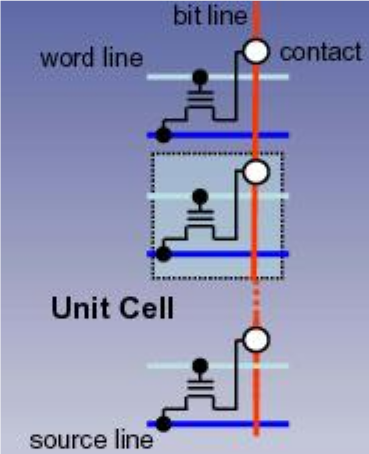
\includegraphics[width=\textwidth]{img/NOR.png}
    \end{minipage}
    \hfill
    \begin{minipage}[b]{0.4\textwidth}
        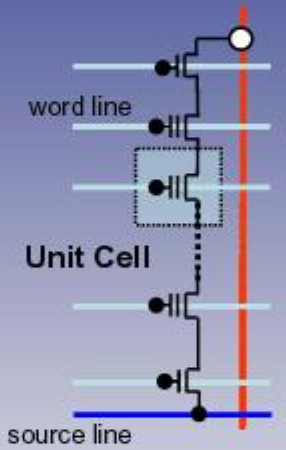
\includegraphics[width=\textwidth]{img/NAND.png}
    \end{minipage}
    \caption*{Nalevo NOR, napravo NAND}
\end{figure}


\subsubsection*{FeRAM}
Konstrukčně obdobné DRAM paměti, ale dielektrikum je tvořeno feroelektrickým materiálem.\\
Informace je zachována i po vypnutí napájení.\\
Uplatnění v průmyslových a bankovních systémech.\\
Výhody oproti FLASH - vyšší počet cyklů mazání($10^16$), vyšší rychlost zápisu, nižší spotřeba.\\
Nevýhody oproti FLASH - malá hustota, limitovaná max kapacita, vyšší cena.
Základem jsou feroelektrické krystaly. Založeno na vystavení feroelektrického krystalu elektrickému poli, centrální atom v mřízce krystalu se vychýlí ve směru elektrického pole. a zapřičiní proudový náraz. Ten je zaznamenán vnitřními obvody a paměť je následně zapnuta. Díky tomu, že atom zůstane vychýlen i po odstranění pole zůstává informace uchována.
Feroelektrický materiál uvnitř feroelektrického kondezátoru v podobě tenkého filmu mezi elektrodami.
\begin{figure} [h!]
    \centering
    \includegraphics*[scale = 0.3]{img/FeRAM.png}
\end{figure}

\subsubsection*{MRAM - Magnetoresistive RAM}
Uplatnění v ukládání dat v uzlech IoT, aplikace strojového učení a umělé inteligenci.\\
Magnetorezistivní jev, změna odporu materiálu vlivem působení magnetického pole. Odpor se mění podle orientace magnetického pole při zápisu bitu.\\
V MRAM se používá tunelová magnetorezistence - TMR. změn R o 30-70\%.\\
TMR nastává na přechodu mezi dvěma feromagnetickými plátky oddělenými tenkým izolátorem. Dielektrická vrstva oxidu hliníku.\\
Každý plátek může být zmangnetizován. \\
Jeden plátek tvoří permanentní magnet s neměnnou orientací magnetického pole.\\
Magnetizace druhého plátku je nastavována vnějším polem tak, aby orientace jeho pole odpovídala zapamatování 1 nebo 0.\\
Paralelní magnetizace je logická 0, antiparalelní magnetizace logická 1.

\begin{figure}[h!]
    \centering
    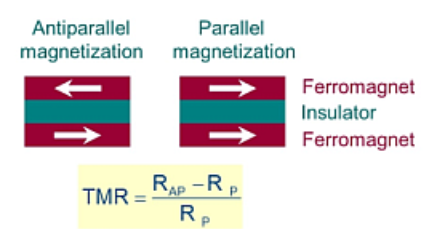
\includegraphics[scale = 0.5]{img/MRAM.png}
\end{figure}

Rychlost srovnatelná s SRAM. Hustota informace jako DRAM. Rychlejší než FLASH, menší spotřeba než DRAM.

Princip: Pokud je směr magnetického pole proměnné feromagnetické vrsty (plátku) stejný s pevně daným směrem spodní vrstvy, je odpor kladený elektrickému proudu malý. Pokud je vzájemná orientace polí opačná, je vertikální elektrický odpor struktury velký. Změna logického stavu z 0 na 1 nebo z 1 na 0 se provádí přivedením sekvence dvou vzájemně posunutých proudových obdélníkových pulsů na dva zápisové vodiče paměťové buňky.\\
Čtení stavu bitu se provádí prostřednictvím jedné společné elektrody a menší speciální čtecí elektrody napojené na protější stranu vertikální struktury.\\
Zapsaný stav 1 - buňka má větší odpor a naopak.\\

\section{Princip a vlastnosti statických pamětí RAM (SRAM) a dynamických pamětí RAM (DRAM), synchronní paměti DRAM (SDRAM).
  Připojování paralelních pamětí SRAM, FLASH ke sběrnicím mikroprocesoru. Adresový dekodér.
  Hierarchie paměti, paměti cache, specializované paměti cache.}

\subsection{SRAM, DRAM a SDRAM}
\subsubsection*{SRAM - Statická RAM}
Paměťová buňka tvořena bistabilním klopným obvodem.\\
Paměťová buňka je rychlá, ale velká – tvořena 6 tranzistory.\\
Využívá se jako procesorová Cache.\\
Výhodou je vysoká rychlost čtení a zápisu. Nevýhodou malá hustota oproti DRAM.\\
Snadné připojení k CPU.\\
\begin{figure}[h!]
    \centering
    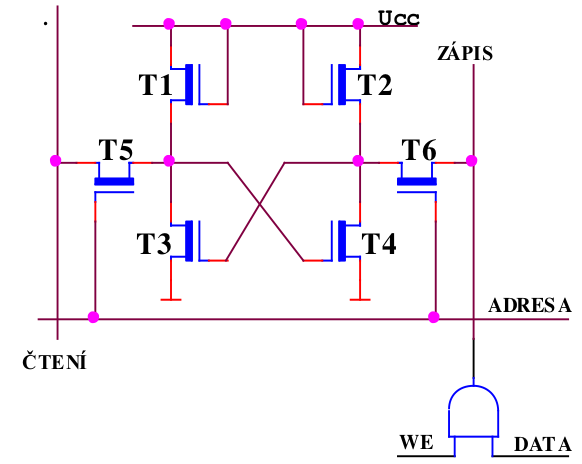
\includegraphics[scale = 0.3]{img/SRAM.png}
\end{figure}

\subsubsection*{DRAM - Dynamická RAM}
K zapamatování informace využívá náboj na kondenzátoru o kapacitě řádově desítky fF (femtofarad $10^{-15}$ F).\\
Paměťová buňka je malá - 1 tranzistor a 1 kondenzátor.\\
Náboj v kondenzátoru je třeba obnovovat, aby nedošlo ke ztrátě informace. Tomuto se říká refresh, je nutno jej provádět každých 64ms\\
Na stejné ploše čipu má DRAM větší kapacitu, než SRAM => nižší cena za 1 bit u paměti SRAM.\\
Kondenzátor se při zápisu nabije nebo vybije přes jednoduchý spínač MOSFET a po určitou dobu udržuje náboj.\\
Napětí na kondenzátoru lze během čtení porovnat s referenčním napětím a rozlišit stav 1 a 0.\\
Adresa do paměti se zavádí ve dvou krocích:
\begin{itemize}
    \item Impulsem RAS\ se zapíše adresa do řádkového registru
    \item Impulsem CAS\ se zapíše adresa do sloupcového registru
\end{itemize}
\begin{figure}
    \centering
    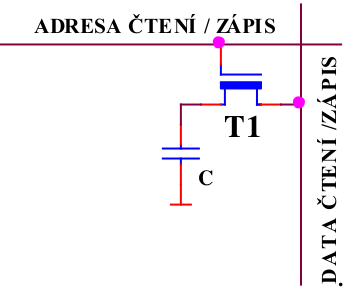
\includegraphics[scale = 0.3]{img/DRAM.png}
\end{figure}

\subsubsection*{SDRAM}
Zavedení synchronizačních (hodinových) impulsů.\\
Všechny vstupní signály jsou náběžnou hranou hodinového impulsu
zapsány do vnitřních registrů.\\
Vnitřní signály se tak mění v přesně definovaných okamžicích a naopak na časování vnějších signálů jsou kladeny podstatně menší nároky než u jednoduché DRAM.\\
Lze na ně zapisovat shluky dat(bytů) - burst reading/writing. Velikosti 1,2,4,8,16B(DDR5) velikost shluku obvykle odpovídá velikosti cache.
Obsahují několik paměťových matic nazývaných banky. Jednotlivé banky mohou pracovat samostatně. Banky jsou dále děleny na řádky(stránky, pages). Dále jsou řádky děleny na sloupce, v každém řádku 1Ki sloupců.\\
Adresa je tvořena:
\begin{itemize}
    \item Adresou skupiny bank: BG0-BG1
    \item Adresou banky: BA0-BA1
    \item Adresou řádku: A0-A14
    \item Adresou sloupce
\end{itemize}

\subsection{Připojování paralelních pamětí SRAM, FLASH ke sběrnicím procesoru}
\begin{itemize}
    \item $A_x$ - adresové sběrnice
    \item $D_x$ - datové sběrnice
    \item MEMR\ - řidicí sběrnice memory read
    \item MEMW\ - řidicí sběrnice memory write
    \item OE\ - output enable
    \item WE\ - write enable
    \item CS\ - chip select - slouží pro výběr paměťového čipu
\end{itemize}
\newpage
\begin{figure}[h!]
    \centering
    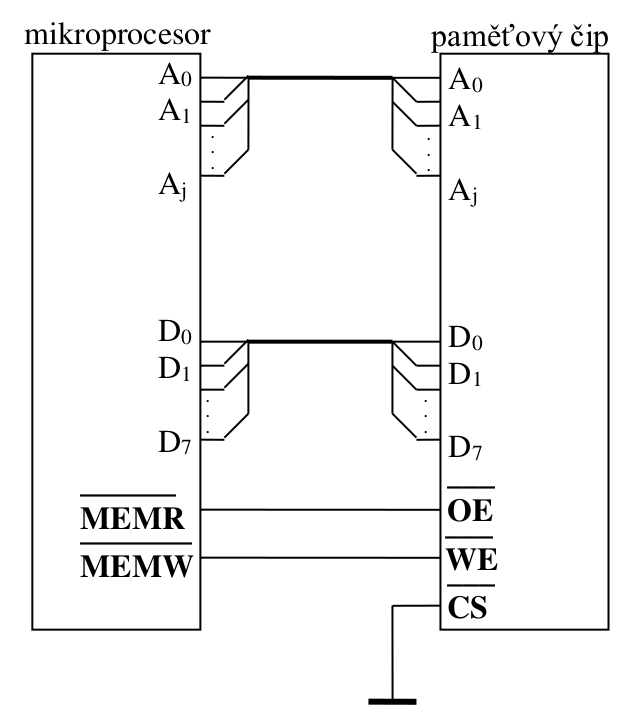
\includegraphics[scale = 0.3]{img/MemConnect.png}
\end{figure}

\subsubsection*{Adresový dekodér}
Binární dekodér zajišťuje rozdělení
paměťového prostoru na jednotlivé čipy.\\
Na základě nejvyšších bitů adresy je aktivován vždy pouze jeden výstup adresového dekodéru, který aktivuje příslušný čip.\\

\begin{figure}[h!]
    \centering
    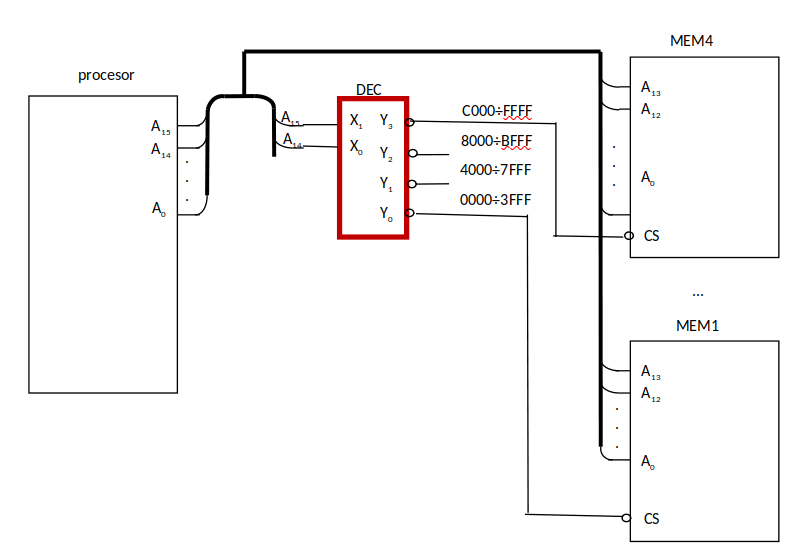
\includegraphics[scale = 0.35]{img/AdrDekoder.png}
\end{figure}
\newpage
\begin{figure}
    \centering
    \includegraphics*[width = \textwidth]{img/AdrDekTab.png}
\end{figure}

\subsection{Hierarchie paměti, paměti cache a specializované cache}
Procesory jsou o několik řádů rychlejší než operační paměť, tudíž musí čekat, což je plýtvání časem.
Chování programů jde popsat pomocí lokalit instrukcí a dat.
\subsubsection*{Časová lokalita instrukcí}
Je-li použita instrukce, dá se očekávat, že se vrzy použije znovu.
\subsubsection*{Prostorová lokalita instrukcí}
Je-li použita instrukce, dá se očekávat, že se vrzy použije instrukce na blízké adrese.

\subsubsection*{Hierarchie paměti}
Schéma VonNeumannova počítače je doplněno o vyrovnávací paměti procesoru takzvané cache, které jsou umístěny mezi procesor a hlavní paměť.
\begin{figure}[h!]
    \centering
    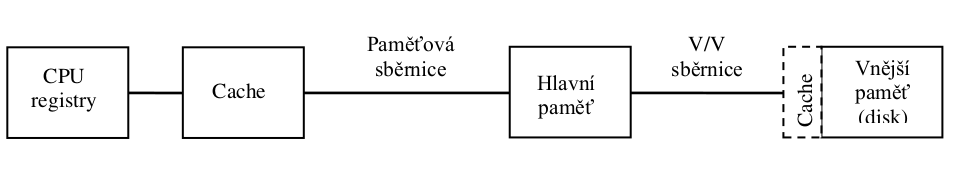
\includegraphics[width = \textwidth]{img/Hierarchie.png}
\end{figure}
Hierarchií rozumíme několik úrovní pamětí různých kapacit a rychlostí. Jsou seřazeny dle kapacity vzestupně a rychlosti sestupně.
\begin{enumerate}
    \item Registry - nejblíže procesoru, stejně rychlé jak procesor, avšak s velmi malou kapacitou
    \item Cache - kapactině jednotky až nižší desítky MB, ale rychlá a drahá SRAM paměť
    \item Hlavní operační paměť
    \item Vnější disk - nejvyšší kapacita, avšak velmi pomalé
\end{enumerate}
\subsubsection*{Cache}
Mezi procesorem a hlavní pamětí. \\
Obsahuje často používané instrukce a data, aby nebylo nutné je číst z hlavní paměti. \\
Když procesor potřebuje číst nebo zapisovat do hlavní paměti, prve se podívá zda tu data jsou, pokud ano pro čtení a ne pro psaní tak data zapíše do cache což je mnohem rychlejší než psaní nebo čtení do/z hlavní paměti. \\
Cache hit - procesor našel v cache, Cache miss - nenašel, hit rate - úspěšnost hitů.\\
Menší cache je rychlejší, ale čím větší je tím má větší hit rate.\\
Dělí se na 3 typy
\begin{itemize}
    \item L1 - nejmenší a nerychlejší, pro každé jádro zvlášť, při přístupu nemusí procesor čekat.
    \item L2 - větší, pomalejší, pro každé jádro zvlášť, při přístupu čeká 1 až 2 hodiné takty.
    \item L3 - největší, společná pro všechny jádra.
\end{itemize}

\subsubsection*{Specializované cache}
Většina moderních procesorů má alespoň 3 nezávislé cache.\\
\begin{itemize}
    \item Instruction cache - pro instrukce
    \item Data cache - pro data procesoru
    \item TLB cache - Translation look-aside buffer cache, zrychluje překlad fyzických adres na fyzické
\end{itemize}

\section{Pojem logická a fyzická adresa, ochrana paměti, memory management unit (MMU). Stránkování (princip, transformace logické adresy na fyzickou, stránkovací tabulka). Virtuální adresový prostor. Zrychlení překladu adres pomocí Translation Look-aside Buffer (TLB).}

MMU - memory mamangement unit. \\
\subsection{Abstrakce paměti}
\subsubsection*{Žádná abstrakce paměti}
Každý proces vidí přímo fyzickou adresu.\\
Paměťový model s kterým pracuje uživatel je fyzická adresa - množina adres od 0 do maximální hodnoty paměti.\\
Využívají kontroléry.\\
\subsubsection*{Abstraktovaná paměti}
Každý proces má svůj vlastní adresový prostor.\\
Musí se zajistit aby stejné adresy v různých procesech odpovídaly jiným fyzickým adresám.\\

\subsection{Logická adresa}
Adresa virtuální s níž pracuje programátor.\\
U jednoduchých procesorů zajišťuje jejich generování přímo procesor. U složitějších procesorů zajišťuje MMU.

\subsection{Fyzická adresa}
Reálná adresa na sběrnici, se kterou pracuje MMU.\\
Na vývodech procesoru je 20-bitová fyzická adresa, která se vytváří tak, že se obsah segmentového registru posune o 4 bity doleva a k ní se lineárně přite offset.
Takto je vytvořen rozsah fyzických adres 0-FFFFFH (0-1MB).\\
Vzniknou překladem logických adres v MMU.\\

\subsection{Ochrana paměti}
\subsubsection*{Segmentace}
Mechanismus správy paměti, který odpovídá uživatelskému pohledu na paměť. \\
Každý program obsahuje data (proměnné), instrukce (kód) a zásobník.\\
Uvedené části programu mají svoje specifické vlastnosti a lze je považovat za relativně samostatné. Proto je lze od sebe oddělit a lze je ukládat do samostatných oblastí paměti, které nazýváme segmenty.\\
Logická adresa segmentu je tvořena dvojicí < číslo segmentu : offset>. Číslo segmentu - určuje začáteční adresu segmentu, nachází se v příslušném segmentovém registru.\\
Z důvodu bezpečnosti pracuje se segmentovými registry a s tabulkami hlavně operační systém, uživatelský program pouze určuje offsetovou část adresy.\\

\subsubsection*{Spojitá alokace}
Rozdělení na pevné délky paměti pro každý proces.
Neefektivní, vznikají prázná místa v paměti.

\subsubsection*{Memory Management Unit}
Zajišťuje oddělení logického a fyzického  adresového prostoru.\\
Ochranu paměti - vzájemné izolování uživatelských procesů, izolování jádra OS a uživatelských procesů.\\
Obsahuje relokační registry.\\
Jednoduché procesory nemají MMU a pracují přímo s fyzickými adresami.\\

\subsubsection*{Stránkování}
Logický prostor je rozdělen na části stejné velikosti, takzvané stránky. Obvyklá velikost je 4KB.\\
Fyzická paměť je rozdělena na rámce. Velikost rámce je stejná jako velikost stránky. \\
Logická adresa se skládá z offsetu, který určuje vzdálenost od začátku stránky a čísla stránky, který určuje číslo stránky. Položky tabulky stránek určují číslo rámce.\\
Položka obsahuje příznak přítomnosti/nepřítomnosti stránky ve fyzické paměti. Realizace pomocí jednoho bitu. Když se nenachází, generuje přerušení(page fault) a OS musí zajistit přesunutí stránky do fyzické paměti z pevného disku.\\
Bity ochrany určují jaké operace jsou se stránkou povoleny. V jednodušším případě pouze 1 bit, 0 je R/W a 1 je pouze R. Sofistikovanější využívá 3 bity, bit povolující čtení, zápis a spouštění kódu ve stránce. \\
Bit odkazu na stránku se nastavuje vždy když je stránka čtena, nebo je do ní zapsáno. Bit pomáhá OS rozhodnout, kterou stránku uvolnit z fyzické paměti, když jsou zaplněny všechny rámce a je požadováno do fyzické paměti umístit další stránku. \\
\begin{figure}[h!]
    \centering
    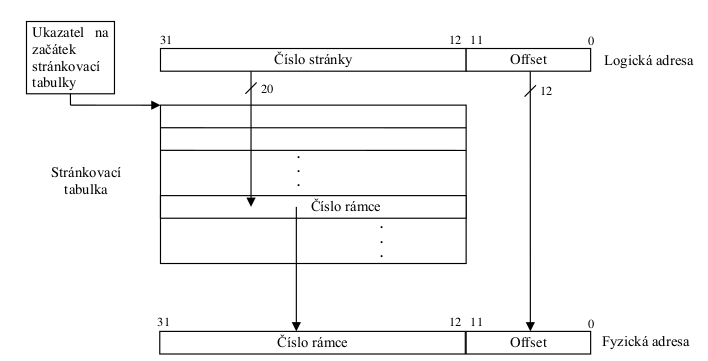
\includegraphics[scale = 0.5]{img/Strankovani.png}
\end{figure}

\subsubsection*{Víceúrovňové stránkovací tabulky}
Většina dnešních počítačových systémů umožňuje pracovat s logickým adresovým prostorem od $2^32$ do $2^64$.
Logickou adresu o velikosti 32 bitů můžeme například rozdělit na 3 části: 10 bitové pole PT1 představující index do stránkovací tabulky první úrovně, 10 bitové pole PT2 představující index do stránkovací tabulky druhé úrovně a 12 bitový offset v rámci stránky. Stránkovací tabulka první úrovně má 2 10 = 1024 položek. Každá stránkovací tabulka druhé úrovně má také 1024 položek, přitom položka tabulky reprezentuje stránku o velikosti 2 12 = 4096 B. Každá tabulka druhé úrovně tedy reprezentuje paměťový prostor 1024*4096 = 4MiB.

\begin{figure}[h!]
    \centering
    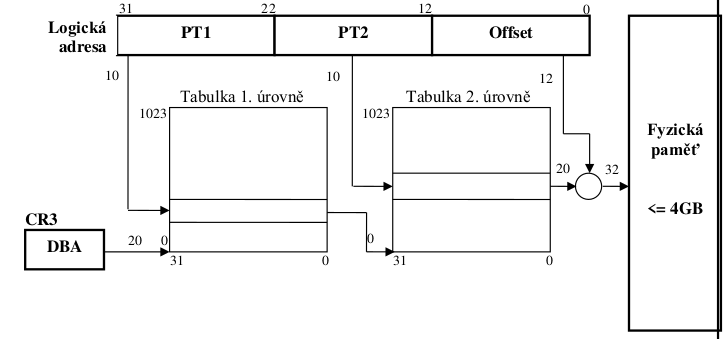
\includegraphics[scale = 0.5]{img/str2.png}
\end{figure}

\subsubsection*{Virtuální adresový prostor}
Oddělení uživatelské logické paměti od fyzické paměti.\\
Metoda zvětšení fyzické paměti ukládáním na pevný disk.\\
Získáme větší prostor než kolik je velikost RAM. Ukládání je velmi pomalé, proto ukládáme pouze to co se nevejde do RAM, nebo je velmi malé.\\
U virtuální paměti se ukládají jen části procesů, kdyby šlo o swapping tak se ukládají celé procesy.\\

\subsubsection*{Translation look-aside buffer}
Slouží ke zrychlení překladu logické adresy na fyzickou. \\
Bez TLB se musíme podívat do paměti 2x, podívání do stránkovací tabulky a podívání do paměti.\\
Typ cache paměti.\\
Jsou v něm uloženy posledně používané lineární adresy a jejich odpovídající fyzické adresy.\\
Nová adresa se prvně hledá v TLB.\\
Většina programů provádí velké množství odkazů do malého počtu stránek.\\
Je součástí MMU. \\